\section{Results under the judges}
\label{sec:judges}

Every judge reorders each system's own fixed top-100 and nothing else (Section~\ref{sec:setup}).
Table~\ref{tab:main} gives \FS{} for the four systems with and without each judge; the paired
comparisons behind it are in Appendix~\ref{app:d5}, the comparable metrics in
Appendix~\ref{app:d6}. The union line is descriptive. The table is the single source for the
statements below; each also cites its macros, so the text and the table cannot drift.

\begin{table}[t]
\centering
\small
\caption{\capMainResult{} $^\dagger$ marks a descriptive union line.}
\label{tab:main}
\coltable{tables/main-result}
\end{table}

\paragraph{The strong cross-encoder lifts every system on every set.} Under J-strong the
standard recipe P10-B gains \deltaStrongPTenBHotpot\pp{} on HotpotQA, \deltaStrongPTenBMusique\pp{} on
MuSiQue and \deltaStrongPTenBMultihop\pp{} on MultiHop-RAG (the exact $p$ of each is in
Appendix~\ref{app:d5}). The same holds for P10-A, P10-C and P14 on all three
sets: all twelve differences are positive. It is also a stronger control than any the line had
before. On HotpotQA, J-strong(P10-B) reaches \fsPctStrongPTenBHotpot{} where P14 without a judge
reaches \fsPctPFourteenHotpot{} (in-sample for P14's weights); on MuSiQue it reaches
\fsPctStrongPTenBMusique{} against P14's \fsPctPFourteenMusique{}; on MultiHop-RAG it reaches
\fsPctStrongPTenBMultihop{} against P14's \fsPctPFourteenMultihop{}, a step far larger than the hop's, which was
negative there. We therefore do not claim that the hop beats a standard judge-equipped recipe.

\paragraph{Does the hop's pool still add under a judge?} This is the comparison J(P14) against
J(P10-B). Under J-strong the label is \texttt{\labelStrongHotpot} on HotpotQA
(\deltaStrongHopHotpot\pp, \winsStrongHopHotpot{} wins, \lossesStrongHopHotpot{} losses) and
\texttt{\labelStrongMusique} on MuSiQue (\deltaStrongHopMusique\pp, \winsStrongHopMusique{} wins,
\lossesStrongHopMusique{} losses), and \texttt{\labelStrongMultihop} on MultiHop-RAG
(\deltaStrongHopMultihop\pp, \winsStrongHopMultihop{} wins, \lossesStrongHopMultihop{} losses). So on the two
Wikipedia benchmarks the hop's candidates carry evidence a strong judge can use, and on news they
do not. Under J-light the labels are \texttt{\labelLightHotpot}, \texttt{\labelLightMusique} and
\texttt{\labelLightMultihop}.

\paragraph{The light cross-encoder helps on Wikipedia, mostly, and hurts on news.} J-light
lifts P10-A and P10-B on HotpotQA (\deltaLightPTenAHotpot\pp, \deltaLightPTenBHotpot\pp) and MuSiQue
(\deltaLightPTenAMusique\pp, \deltaLightPTenBMusique\pp), is flat on P10-C on MuSiQue
(\deltaLightPTenCMusique\pp) and \emph{lowers} P14 on both (\deltaLightPFourteenHotpot\pp,
\deltaLightPFourteenMusique\pp). On MultiHop-RAG it lowers every system, P10-B by
\deltaLightPTenBMultihop\pp. Its input window truncated \truncCountLightMultihop{} pairs on news, against
\truncCountLightHotpot{} on HotpotQA, and no pair for the other two judges (Table~\ref{tab:judgecost});
we did not test whether that explains the news result.

\begin{figure}[t]
\centering
% Generated by `cer p17-tables`; do not edit. Coordinates are written from the artifacts.
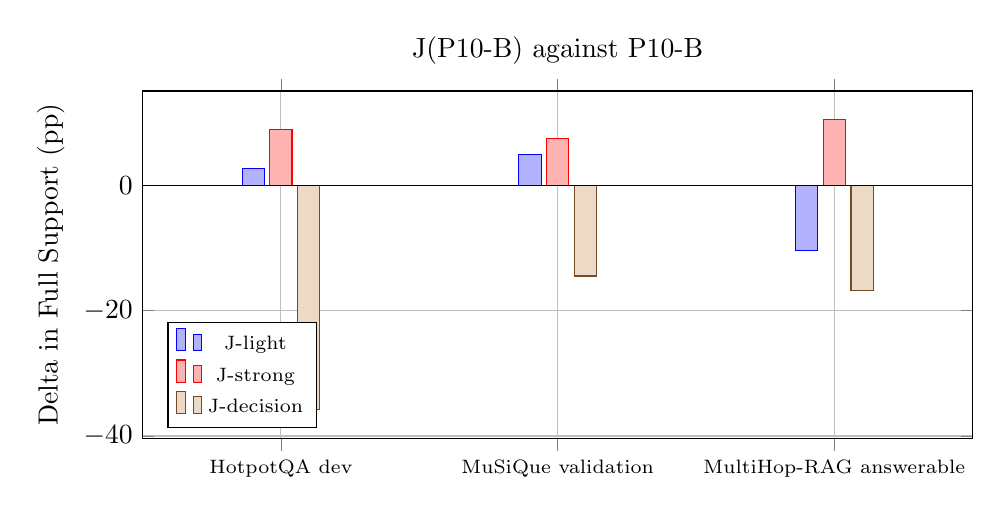
\begin{tikzpicture}
\begin{axis}[ybar, width=\columnwidth, height=6cm, bar width=8pt, enlarge x limits=0.25, xtick={0,1,2}, xticklabels={{HotpotQA dev},{MuSiQue validation},{MultiHop-RAG answerable}}, x tick label style={font=\scriptsize}, ylabel={Delta in Full Support (pp)}, grid=major, legend pos=south west, legend style={font=\scriptsize}, title={J(P10-B) against P10-B}]
\addplot coordinates {(0,2.62) (1,4.96) (2,-10.42)};
\addlegendentry{J-light}
\addplot coordinates {(0,8.94) (1,7.45) (2,10.42)};
\addlegendentry{J-strong}
\addplot coordinates {(0,-35.84) (1,-14.48) (2,-16.81)};
\addlegendentry{J-decision}
\draw (axis cs:-1,0) -- (axis cs:3,0);
\end{axis}
\end{tikzpicture}

\caption{Change in \FS{} when each judge reorders the standard recipe P10-B, in percentage
points, per set. Written from the artifacts.}
\label{fig:delta}
\end{figure}

\paragraph{The bi-encoder decision judge hurts everywhere: a negative result.} J-decision
lowers every system on every set, P10-B by \deltaDecisionPTenBHotpot\pp{} on HotpotQA,
\deltaDecisionPTenBMusique\pp{} on MuSiQue and \deltaDecisionPTenBMultihop\pp{} on news
(Figure~\ref{fig:delta}); J-decision(P10-B) wins \winsCrossDecisionVsStrongHotpot{} questions and loses
\lossesCrossDecisionVsStrongHotpot{} against J-strong(P10-B) on HotpotQA. Its hop labels are
\texttt{\labelDecisionHotpot}, \texttt{\labelDecisionMusique} and \texttt{\labelDecisionMultihop},
which are small differences between two bad orders. We read this as a measurement of this
\emph{use} of the model, not of the model: it is a bi-encoder that compares two separate
embeddings and cannot weigh a candidate's words against the question's the way a cross-encoder
does; it was designed for agent decisions, has no published passage-retrieval benchmark, and was
used here zero-shot with the question alone as its state and no instruction. We cannot separate
``it does not rank evidence'' from ``this usage does not suit it'', and the preregistration forbade
trying another prompt.

\paragraph{Determinism.} The two cross-encoders are deterministic to float noise: re-scoring
\detQuestionsLightHotpot{} questions at batch size one changed the order of \detOrderChangedLightHotpot{} of them,
with a largest score difference of \detMaxDiffLightHotpot{} for J-light and \detMaxDiffStrongHotpot{} for
J-strong on HotpotQA. J-decision is not: its encoder runs in bfloat16 (a 24~GB card cannot hold
it in float32) and the serving engine batches sequences itself, so the same re-scoring changed the order of
\detOrderChangedDecisionHotpot{} of \detQuestionsDecisionHotpot{} questions, with a largest difference of \detMaxDiffDecisionHotpot{} in the
score. Its figures are therefore one realization of the model; we did not measure how much a
second pass would move \FS, so the size of that effect is unknown.

\begin{figure}[t]
\centering
% Generated by `cer p17-tables`; do not edit. Coordinates are written from the artifacts.
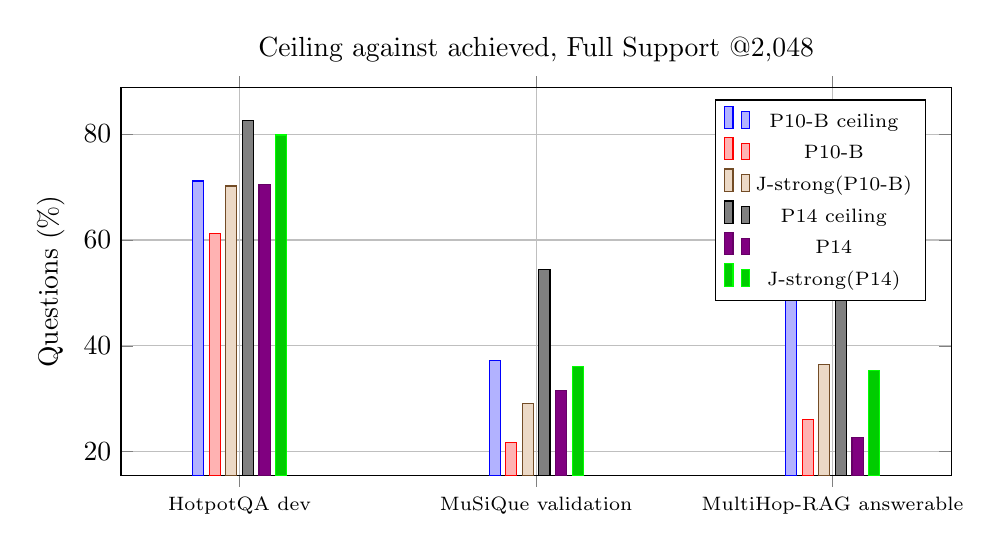
\begin{tikzpicture}
\begin{axis}[ybar, width=\columnwidth, height=6.5cm, bar width=4pt, enlarge x limits=0.2, xtick={0,1,2}, xticklabels={{HotpotQA dev},{MuSiQue validation},{MultiHop-RAG answerable}}, x tick label style={font=\scriptsize}, ylabel={Questions (\%)}, grid=major, legend pos=north east, legend style={font=\scriptsize}, title={Ceiling against achieved, Full Support @2,048}]
\addplot coordinates {(0,71.13) (1,37.24) (2,51.44)};
\addlegendentry{P10-B ceiling}
\addplot coordinates {(0,61.26) (1,21.68) (2,26.03)};
\addlegendentry{P10-B}
\addplot coordinates {(0,70.20) (1,29.13) (2,36.45)};
\addlegendentry{J-strong(P10-B)}
\addplot coordinates {(0,82.63) (1,54.49) (2,50.78)};
\addlegendentry{P14 ceiling}
\addplot coordinates {(0,70.55) (1,31.49) (2,22.75)};
\addlegendentry{P14}
\addplot coordinates {(0,79.82) (1,36.04) (2,35.34)};
\addlegendentry{J-strong(P14)}
\end{axis}
\end{tikzpicture}

\caption{The judge ceiling for the standard recipe and for P14: the share of questions whose
gold paragraphs all lie inside the system's top-100, beside what \FS{} the system achieves
without a judge and under J-strong.}
\label{fig:ceiling}
\end{figure}

\paragraph{How much of the room does a judge close?} A reorder cannot recover gold that lies outside the
pool; Figure~\ref{fig:ceiling} shows how far each system is from that bound. On HotpotQA, J-strong takes P10-B
from \fsPctPTenBHotpot{} to \fsPctStrongPTenBHotpot{} against a ceiling of
\ceilPTenBHotpot{} questions, and P14 to \fsPctStrongPFourteenHotpot{} (\fsStrongPFourteenHotpot{} questions
against a ceiling of \ceilPFourteenHotpot{}), only \ceilFailStrongPFourteenHotpot{} questions short of what its pool
allows. The union pool under J-strong reaches \fsStrongUnionHotpot{} questions: \textbf{P14 under J-strong
is at the union pool's level on HotpotQA}, so the hop's pool is already the best pool of the four there. On
MuSiQue P14's pool is the bigger one (a ceiling of \ceilPFourteenMusique{} against \ceilPTenBMusique{} for
P10-B), and under J-strong it reaches \fsStrongPFourteenMusique{} questions against \fsStrongUnionMusique{}
for the whole union pool; a hypothesis is that a larger pool lets a judge be wrong more often. On news P10-B's own pool
holds the gold of more questions than P14's (\ceilPTenBMultihop{} against \ceilPFourteenMultihop{}),
the opposite of the Wikipedia sets, and the union pool under J-strong is the best
line there (\fsStrongUnionMultihop{} questions). The ceilings are exploratory diagnostics computed from the gold.
The budget curve (Appendix~\ref{app:more}) shows that under J-strong the first 512 tokens already carry
\fsBudgetFiveTwelveStrongPFourteenHotpot{}\% on HotpotQA for P14, against \fsBudgetFiveTwelvePFourteenHotpot{}\%
without a judge.

\paragraph{Cost beside every figure.}
\begin{table}[t]
\centering
\small
\caption{\capJudgeCost}
\label{tab:judgecost}
\coltable{tables/judge-cost}
\end{table}
Table~\ref{tab:judgecost} gives pairs, throughput and attributable cost on one rented RTX~4090. J-light
scored all of HotpotQA's pairs in \wallSecLightHotpot{} s for \usdLightHotpot{} USD; J-strong took
\wallSecStrongHotpot{} s and \usdStrongHotpot{} USD; J-decision took \wallSecDecisionHotpot{} s and
\usdDecisionHotpot{} USD there. J-decision's wall time is dominated by embedding every distinct unit of
the pool once, which is why its pairs per second differ by an order of magnitude across the sets. The
three judges together cost \usdGpuAttributable{} USD of attributable GPU time; the whole rented session ran
\sessionHours{} h \sessionMinutes{} min and cost \usdSession{} USD by the balance recorded before and after
(derived). At query time a cross-encoder judge scores a pool of about \poolMeanHotpot{} pairs per
question on HotpotQA; the line's own systems, which call no model beyond the first Dense pass, are
never claimed to match a judge's quality at their cost.
